\labsection{1}{Search Foundations on an Airline Network}{sec:lab01-search}

\begin{labproject}{Build and compare BFS, DFS, and Uniform-Cost Search}
\textbf{Read first.} Chapter~\ref{ch:uninformed}. Chapters~\ref{ch:toolkit} and~\ref{ch:git-submission} set up your tools.\\
\textbf{Goal.} Run BFS, DFS and UCS on one cleaned graph, verify every path, and explain why the algorithms disagree.\\
\textbf{Scenario.} Build a route planner over real airline connections and compare route quality with search effort.\\
\textbf{Data.} \texttt{all\_datasets/lab01-03\_airports.csv} and \texttt{lab01-03\_routes.csv}.\\
\textbf{Notebook.} \texttt{all\_experiments/lab01\_search\_foundations\_worked.ipynb}; Labs 1--3 share \texttt{all\_experiments/utils/}.\\
\textbf{Hand in.} The executed notebook, the \texttt{results/lab01/} folder and a short conclusion, as listed in the checklist at the end of this sheet.
\end{labproject}

\begin{labmode}
\begin{enumerate}
  \item Activate your course environment (Chapter~\ref{ch:toolkit}) and confirm that both data files are in \texttt{all\_datasets/}.
  \item Warm up on the robot's maze, which needs no data. From the course folder, run the command below. Its last line must read \texttt{Every number above matches the book.}
  \item Start Jupyter from \texttt{all\_experiments/}, open the notebook, and choose \textbf{Restart Kernel and Run All Cells}. Everything runs in a few seconds.
\end{enumerate}
\begin{lstlisting}[style=utpterminal]
python all_experiments/demo_robot_maze.py
cd all_experiments
jupyter lab
\end{lstlisting}
Prefer a plain script? From the course folder, \texttt{python all\_experiments/lab01\_search\_foundations\_worked.py} runs the same code and writes the same evidence.
\end{labmode}

\courselabflow{Clean routes}{Choose frontier}{Search routes}{Verify paths}


\labroutine

\begin{yourturn}
\textbf{Warm-up on paper.} Before touching the airline data, trace BFS and UCS by hand on the seven-node graph of \figref{fig:ucs-vs-bfs}, writing out the frontier after each expansion. You will check your trace with code at the end of this sheet.
\end{yourturn}

\textbf{Setup.} Run the imports and path setup first, and keep this kernel state for the later questions. In the script version the first seven lines also set the working directory, so that relative paths resolve.
\lstinputlisting[style=utppython,firstline=1,lastline=7]{all_experiments/lab01_search_foundations_worked.py}
\lstinputlisting[style=utppython,firstline=8,lastline=19]{all_experiments/lab01_search_foundations_worked.py}

\begin{labquestion}{1}{Load and validate the graph}
Load the airport and route files, keep only airports with a valid IATA code and coordinates, drop routes whose endpoints are unusable, and collapse duplicate routes. Report how many rows survive each step and show the three standard queries.
\end{labquestion}
\begin{labanswer}
\courselabtrace{One graph, different objectives}{BFS}{FIFO frontier; minimise hops}{UCS}{Priority by accumulated kilometres}{Check}{Every consecutive edge must exist}

\lstinputlisting[style=utppython,firstline=21,lastline=25]{all_experiments/lab01_search_foundations_worked.py}
\begin{refoutput}
\begin{lstlisting}[style=utpterminal]
airport_rows         10668      valid_airports        6464
route_rows           67663      unique_valid_routes  37337
removed_route_rows   30326
Queries:  Q1 KUL -> KEF     Q2 SIN -> EZE     Q3 NRT -> CPT
\end{lstlisting}
\end{refoutput}

\textbf{What it means.} Of 10,668 airport rows, 6,464 have a usable code and coordinates; of 67,663 route rows, 37,337 unique directed routes connect two usable airports. Every algorithm below runs on this same graph, so their results can be compared.
\end{labanswer}

\begin{labquestion}{2}{Define the edge cost}
BFS and DFS count every route as one step. UCS needs a number: the great-circle (Haversine) distance in kilometres between the two airports. Show the first five routes out of KUL with their distances, and the straight-line distance from KUL to KEF.
\end{labquestion}
\begin{labanswer}
\lstinputlisting[style=utppython,firstline=27,lastline=33]{all_experiments/lab01_search_foundations_worked.py}
\begin{refoutput}
\begin{lstlisting}[style=utpterminal]
KUL has 112 outgoing routes
Great-circle distance KUL -> KEF: 11,316 km (no direct route exists)
\end{lstlisting}
\end{refoutput}

\textbf{What it means.} Each edge carries the distance between its endpoints, computed once when the graph is built. Counting steps (BFS, DFS) and summing kilometres (UCS) are two different questions asked of the same graph.
\end{labanswer}

\textbf{Connect it to the chapter.} The next question runs the loop below three times. Only the highlighted box differs between the three algorithms.
% Reused from chapters/01-uninformed-search.tex
\begin{labvisual}{Recall the chapter model}
\begin{labgraphic}
\begin{tikzpicture}[font=\small]
\node[utpbox,minimum width=2.3cm] (start) at (0,0) {Start\\state};
\node[utpbox,minimum width=2.6cm,fill=UTPPaleOrange,draw=UTPOrange,line width=1pt]
  (pick) at (3.6,0) {\textbf{Select from}\\\textbf{frontier}};
\node[utpbox,minimum width=2.4cm] (goal) at (7.2,0) {Goal\\test?};
\node[utpbox,minimum width=2.6cm,fill=UTPPaleTeal,draw=UTPGreen] (done) at (10.7,0) {Return\\the path};
\node[utpbox,minimum width=2.6cm] (expand) at (7.2,-2.1) {Generate\\successors};
\node[utpbox,minimum width=2.6cm] (vis) at (3.6,-2.1) {Not already\\seen?};

\draw[utparrow] (start)--(pick);
\draw[utparrow] (pick)--(goal);
\draw[utparrow] (goal)--(done) node[midway,above,utplabel,color=UTPGreen] {yes};
\draw[utparrow] (goal)--(expand) node[midway,right,utplabel,color=UTPRed] {no};
\draw[utparrow] (expand)--(vis);
\draw[utparrow] (vis) -- (pick) node[midway,right,utplabel,color=UTPGreen] {keep};
\node[utplabel,anchor=south,align=center,color=UTPOrange] at (3.6,0.72)
  {\textbf{the only line that changes:} FIFO / LIFO / min-cost};
\node[utplabel,anchor=east,align=right] at (2.15,-2.1) {discard\\duplicates};
\end{tikzpicture}
\end{labgraphic}\end{labvisual}


\begin{labquestion}{3}{Run BFS, DFS and UCS on the three standard queries}
Record path, hops, distance, expanded nodes, maximum frontier and runtime for every algorithm and query, and save the table as \texttt{metrics.csv}. \emph{Predict first:} which algorithm will expand the most airports, and which will use the most legs?
\end{labquestion}
\begin{labanswer}
\lstinputlisting[style=utppython,firstline=35,lastline=44]{all_experiments/lab01_search_foundations_worked.py}
\begin{refoutput}
\begin{lstlisting}[style=utpterminal]
query algorithm hops        km expanded max_frontier
Q1    BFS          2  12274.32      284         1679
Q1    DFS         23  41767.82     2112          859
Q1    UCS          4  11461.35     1851          616
Q2    BFS          2  21976.11      233         1629
Q2    DFS         39  65213.84      904          858
Q2    UCS          3  17817.36     3002          620
Q3    BFS          2  19005.89      173         1727
Q3    DFS         64  91541.43     1414          785
Q3    UCS          3  14813.32     3042         1018
\end{lstlisting}
\end{refoutput}

\textbf{What it means.} BFS always returns the fewest hops (two legs on every query), UCS always returns the shortest distance, and DFS returns a long, winding route because it follows the first neighbour deeply. Expanded-node counts are the stable measure of effort; runtimes vary from machine to machine.
\end{labanswer}

\begin{labquestion}{4}{Verify every path independently}
A reported path is only evidence if it can be checked. Confirm that every consecutive pair of airports in every path is a real route, and recompute each path cost by summing the edge distances.
\end{labquestion}
\begin{labanswer}
Here is what the verification loop does for one path:
\courselabtrace{Verify an airline path independently}{1. Input / state}{Split the saved path into airport codes; edge\_km maps each source to its neighbours and distances.}{2. Operation}{For every adjacent pair a, b, confirm b is in edge\_km[a], then add edge\_km[a][b].}{3. Check}{Compare the sum with path\_cost\_km; len(path) - 1 is the hop count.}


\lstinputlisting[style=utppython,firstline=46,lastline=54]{all_experiments/lab01_search_foundations_worked.py}
\begin{refoutput}
\begin{lstlisting}[style=utpterminal]
Verified 9 paths: every leg exists and every cost matches its edge sum
\end{lstlisting}
\end{refoutput}

\textbf{What it means.} All nine paths use real routes and their costs equal the sum of their edge distances, so the metrics table can be trusted. The loader already removed unusable endpoints, yet verification still checks the returned edges: a bug in the search would show up here.
\end{labanswer}

\begin{labquestion}{5}{Compare the objectives}
Show hops and distance side by side for the three algorithms. Then run DFS again with every neighbour list reversed, to show that its answer depends on neighbour order.
\end{labquestion}
\begin{labanswer}
\lstinputlisting[style=utppython,firstline=56,lastline=62]{all_experiments/lab01_search_foundations_worked.py}
\begin{refoutput}
\begin{lstlisting}[style=utpterminal]
Q1 DFS: 23 hops with the original order, 8 with the reversed order
Q2 DFS: 39 hops with the original order, 41 with the reversed order
Q3 DFS: 64 hops with the original order, 39 with the reversed order
\end{lstlisting}
\end{refoutput}

\textbf{What it means.} BFS minimises the number of legs, so a two-leg route through a distant hub (KUL $\rightarrow$ AMS $\rightarrow$ KEF) wins even though UCS finds a four-leg route that is over 800~km shorter. Fewest legs and fewest kilometres are different objectives. DFS changes its answer as soon as the neighbour order changes, because it commits to the first branch it sees; it guarantees neither objective.
\end{labanswer}

\begin{labquestion}{6}{Save the evidence}
Plot the three KUL $\rightarrow$ KEF routes and save the figure next to \texttt{metrics.csv}.
\end{labquestion}
\begin{labanswer}
\lstinputlisting[style=utppython,firstline=64,lastline=68]{all_experiments/lab01_search_foundations_worked.py}
\begin{labvisual}{Reference plot from the supplied notebook}
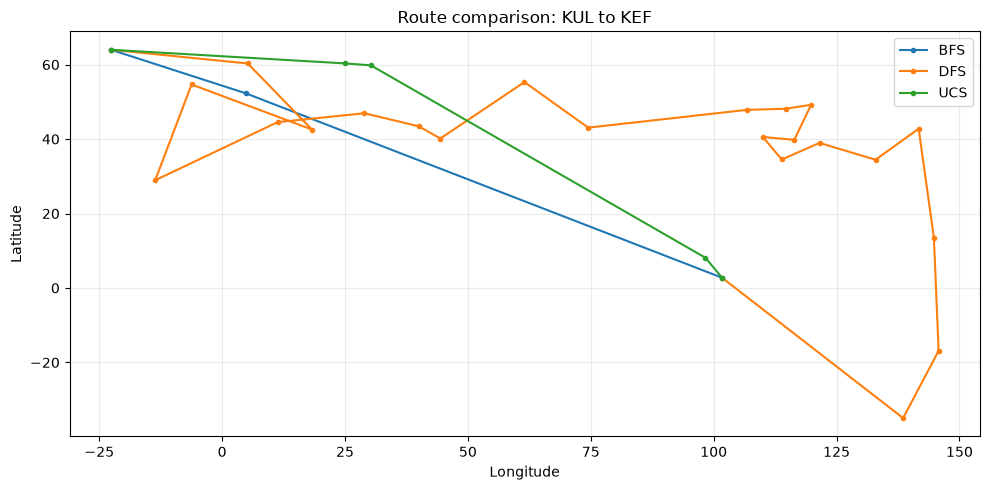
\includegraphics[width=.88\linewidth,height=5cm,keepaspectratio]{labs/visuals/01-notebook-reference.png}
\end{labvisual}
\begin{refoutput}
\begin{lstlisting}[style=utpterminal]
Saved: ['metrics.csv', 'route_comparison.png']
\end{lstlisting}
\end{refoutput}

\textbf{Read the result.} Regenerate this plot rather than copying it. Check the axes and the three routes; this saved figure is a reference, not evidence of your own run.
\end{labanswer}

\begin{yourturn}
Add new cells at the end of the notebook for these three tasks, and record your numbers before reading the expected findings.
\begin{enumerate}
  \item \textbf{Try a new query.} Run all three algorithms from \texttt{JFK} to \texttt{SYD} and record hops, kilometres and expansions.
  \item \textbf{Does direction matter?} Run BFS and UCS from \texttt{KEF} back to \texttt{KUL} and compare with the outward results. Is the best route back the same route reversed?
  \item \textbf{Check your warm-up.} Type in the graph of \figref{fig:ucs-vs-bfs} and compare with your hand trace. Then remove the edge from D to G and predict what BFS returns.
\end{enumerate}
\begin{lstlisting}[style=utppython]
tiny = {"A": [("B", 1.0), ("C", 4.0)], "B": [("D", 3.0), ("E", 2.0)], "C": [("F", 5.0)],
        "D": [("G", 4.0)], "E": [("G", 1.0)], "F": [("G", 2.0)], "G": []}
print(bfs(tiny, "A", "G").path, ucs(tiny, "A", "G").path)
\end{lstlisting}
\end{yourturn}

\begin{expectedfindings}
\begin{enumerate}
  \item BFS: 2 hops, 23,093~km via AUH, 537 expanded. DFS: 45 hops, 64,251~km. UCS: 2 hops, 16,035~km via LAX, 3,097 expanded. BFS stops at the first two-leg route it meets, 7,000~km too long.
  \item BFS: 2 hops via AMS, 12,274~km. UCS: 4 hops via HEL, LED and TAS, 11,478~km, which is not the outward UCS route reversed. Routes are directed, so a route out does not guarantee the same route back.
  \item BFS returns A--B--D--G at cost 8 and UCS returns A--B--E--G at cost 4. With the edge from D to G removed, BFS also returns A--B--E--G, because that is now the first three-edge route it reaches.
\end{enumerate}
\end{expectedfindings}

\begin{troubleshoot}
\begin{description}
  \item[\texttt{ModuleNotFoundError: utils}] Jupyter was not started from \texttt{all\_experiments/}. Restart it from there, or run the script from the course folder.
  \item[\texttt{FileNotFoundError}] A data file is missing or misnamed. Match Chapter~\ref{ch:toolkit}'s names, capitals too.
  \item[Different counts from the reference] Use the supplied data files and an unedited \texttt{utils/core.py}. Runtimes vary by machine; hops, kilometres and expansions should not.
\end{description}
\end{troubleshoot}

\begin{verification}
\begin{itemize}
  \item The cleaned graph has 6,464 usable airports and 37,337 unique directed routes.
  \item Every BFS, DFS and UCS path uses real routes, and its cost is the sum of its legs.
  \item BFS returns the fewest hops and UCS the shortest distance on every query; UCS finds the 11,461~km KUL$\to$KEF route.
  \item Reversing the neighbour order changes the DFS route, and you can explain why.
  \item \texttt{results/lab01/} holds \texttt{metrics.csv} and \texttt{route\_comparison.png}.
\end{itemize}
\end{verification}

\begin{labdeliverable}
\begin{itemize}
  \item Restart the kernel and run all cells without errors.
  \item Submit the executed notebook, including your \emph{Your turn} cells, and the generated \texttt{results/lab01/} folder.
  \item Add a short conclusion: which method minimises hops, which minimises distance, why DFS changes with neighbour order, and which effort measure is comparable across computers.
\end{itemize}
\end{labdeliverable}
